\documentclass[a4paper]{jpconf}
\usepackage{graphicx}
\begin{document}
\title{CLARA: CLAS12 Reconstruction and Analysis Framework}

\author{V Gyurgyan$^1$, S Mancilla$^2$ and R Oyarz\'un$^2$}
\address{$ˆ1$ Thomas Jefferson National Accelerator Facility, Newport News, VA, USA}
\address{$ˆ2$ Universidad T\'ecnica Federico Santa Mar\'ia, Valpara\'iso, Chile}

\ead{gurjyan@jlab.org}

% {\vspace{1em} \hspace{2em}\hspace{2em}\\ % Author names
% {\smaller gurjyan@jlab.org\hspace{4em}smancill@jlab.org\hspace{4em}oyarzun@jlab.org}} % Author email addresses

\begin{abstract}
  In this paper we present SOA based
  CLAS12 event Reconstruction and Analyses (CLARA) framework.
  CLARA design focus is on two main traits:
  real-time data stream processing,
  and service-oriented architecture (SOA)
  in a flow based programming (FBP) paradigm.
  Data driven and data centric architecture of CLARA presents an environment
  for developing agile, elastic, multilingual data processing applications.
  The CLARA framework presents solutions
  capable of processing large volumes of data interactively
  and substantially faster than batch systems.
\end{abstract}

\section{Introduction}

Software systems,
including physics data processing (PDP) applications,
have a distinct component based structure.
Most data processing applications can be described
as a combination of, more or less, independent software units
that are cooperating to achieve data processing goals.
These components in most cases require different optimization criteria
to increase performance of the overall data processing application.
It is arguable difficult to optimize functionally different components
of an application within the same process.
The resulting code becomes bloated,
less readable, difficult to test, debug and maintain.
We think that by designing a PDP application,
based on independent (or loosely coupled), specialized software components as processes
much needed agility and efficiency can be achieved.
Under ``loose coupling'' we assume that
components do not have interdependences other than a data interface.
Thus data processing application components can be considered
as service providers that offer their services through a defined data interface.

\section{Basic Concepts}

The CLARA framework uses SOA\cite{soa} to enhance
the efficiency, agility, and productivity of data processing applications.
Services are the primary means through which
data processing logic is implemented.
CLARA application services are running in a context that is agnostic
to the global data processing application logic.
Services are loosely coupled
and can participate in multiple algorithmic compositions.
Legacy processes or applications can also be presented as services
and integrated into a data processing application.
Services can be linked together
and presented as one, complex, composite service.
This framework provides a federation of services,
so that service-based data processing applications can be united
while maintaining their individual autonomy and self-governance.
CLARA is a multilingual framework that supports services
written in Java, Python and C++ languages.

\subsection{Design architecture}

CLARA architecture consists of three layers,
illustrated in Figure~\ref{fig:design}.
The first layer is the service-bus that provides an abstraction
of the xMsg publish-subscribe messaging system\cite{xmsg}.
xMsg is using the ZeroMQ\cite{zmq} socket library
and implements messaging patterns like
topic pub-sub, workload distribution, and request-response.
Every service from the service layer
or component from the orchestration-layer
communicates via the service-bus,
which acts as a messaging tunnel between CLARA components.
The service-layer houses the inventory of services
used to build data processing applications.
An administrative registration service stores information
about every registered service in the service layer,
including address, description and operational details.

\begin{figure}[!h]
  \begin{center}
    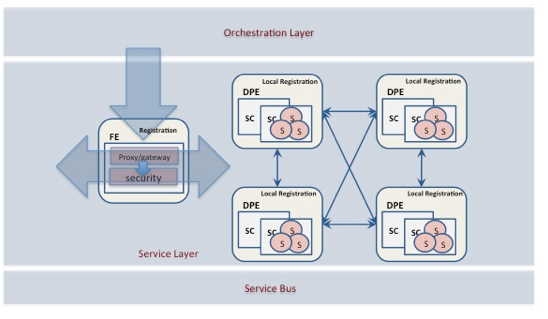
\includegraphics[width=0.6\textwidth]{figures/design}
  \end{center}
  \caption{CLARA architecture:
    Front-End~DPE~(FE),
    Data~Processing~Environment~(DPE),
    Service~Container~(SC),
    Service~(S).}
  \label{fig:design}
\end{figure}

The orchestration of data analyses applications is accomplished by the
application controller (orchestrator), which resides in the
orchestration-layer.
Front-End (FE) is a specialized data processing environment (DPE) that houses
a master registration service on top of the global registration database.
The growing need to fuse, correlate and process widely distributed data in the
CLARA environment will undoubtedly demand data security measures.
CLARA provides normative data-proxy and security services
that can be deployed in the FE.
CLARA security services implement user authentication, data encryption and
transient data envelope integrity.

\subsection{Data envelope}

The CLARA framework provides developers
the ability to interact with services
using the publish-subscribe message exchanges.
In a distributed communication model,
success largely depends on the design of the message structure:
a communication envelope that describes not only transferred data,
but also communication and service operational details.
In order for a service communication to be truly useful,
every service has to share/use the same vocabulary
for expressing the communication details (i.e.~common message-interface).
CLARA transient data envelope is the main message interface between services.
The mutual understanding and acceptance of this object
couples the framework services.
The CLARA data envelope is illustrated in the Figure~\ref{fig:msg}.

\begin{figure}[!h]
  \begin{center}
    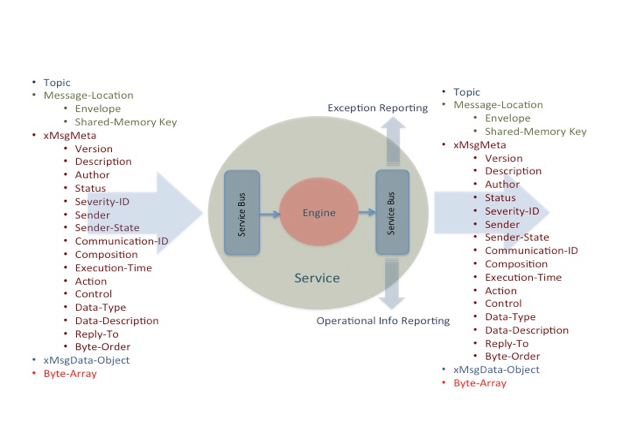
\includegraphics[width=0.65\textwidth]{figures/msg}
  \end{center}
  \caption{CLARA data envelope:
    Envelope can have two or 4-part configuration
    based on the data transferred modes between local or remote services.
    Local: 1)~topic, 2)~shared-memory~key.
    Remote: 1)~topic, 2)~``envelope'', 3)~xMsg~metadata, 4)~serialized~object.}
  \label{fig:msg}
\end{figure}

\subsection{Basic components}

The CLARA platform is composed of
multiple distributed data processing environments (DPE).
DPE provides a run-time environment for services and service-containers
and allows several services to concurrently execute on the same environment.
The use of shared memory prevents unnecessary copying of the data
during service communications.
The DPE runs one or many service-containers
that are designed for logical groupings of services.
Service-containers and services may also be distributed
across multiple computing nodes for the purposes of scaling horizontally
to handle increased data volume.
CLARA application orchestrator can start service-containers in a specified DPE,
and monitor and track functionality of services
by subscribing to specific events from a service-container,
reporting the number of requests to a specific service,
as well as notifying when a successful execution of a particular service
(or its failure) has occurred.
Each service-container deploys one or many services,
presenting their computing algorithms encapsulated in service-engines.
CLARA service implements SOA SaaS as a way of delivering on-demand,
ready-made data processing solutions (service-engines) as CLARA services.

\begin{figure}[!h]
  \begin{center}
    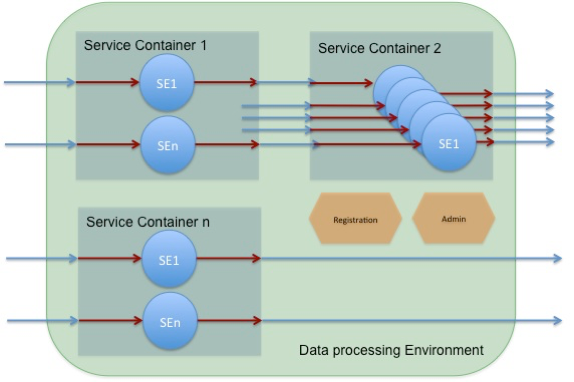
\includegraphics[width=0.45\textwidth]{figures/dpe}
  \end{center}
  \caption{CLARA basic components:
    services~(SE1,~SEn) and
    data streams (arrows).}
  \label{fig:dpe}
\end{figure}

The CLARA data processing application user uses a \textit{service},
but does not control the operating system,
hardware or network infrastructure on which they are running.
The quality of the data-processing application
(including syntactic, semantic qualities, and performance)
depends highly on the quality of constituent service,
delegating a request to its engine.
It is, therefore, critical to test and validate a \textit{service-engine}
before deploying it as a CLARA service.
\textit{Service-engines} must be validated with respect to workflow,
thread-safety, integrity, reliability, scalability, availability, accuracy,
testability and portability.
The DPE also contains a proxy for service connections,
eliminating direct connections between services.
The use of the proxy solves service dynamic discovery problems.
The DPE proxy acts like a simple stateless message switch
(much like an HTTP proxy).
Each \textit{service-container} running in a DPE
contains the map of deployed \textit{service} objects.
Every \textit{service} object subscribes to service requests
and processes the request
by getting the \textit{service-engine} object from the object pool,
and executing the user provided engine in a separate thread.


\subsection{Resource Discovery}

The core of the CLARA registration and discovery mechanism
is the normative registration service
that the services and service containers are registering with.
The registration service, which is started within the DPE,
functions as a naming and directory facility to uncover services.
Services and service-containers in the CLARA registry are described
using unique names, types and descriptions of their functionalities.
The service is advertised by its service description in the registry.
Querying the name and a service functional description
defines the service discovery process.
Registration database is duplicated in the front-end DPE (FE),
controlled by the master registration service.
Each registration service periodically pushes its entire database to the FE.

\begin{figure}[!h]
  \begin{center}
    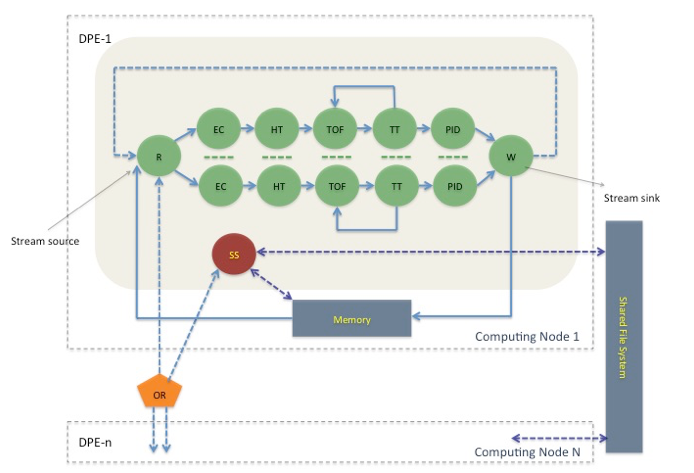
\includegraphics[width=0.75\textwidth]{figures/clas-rec}
  \end{center}
  \caption{CLAS12 data processing application.
    Services:
    stream~builder~(R),
    stream~writer~(W),
    electromagnetic-calorimeter reconstruction~(EC),
    hit~based tracking~(HT),
    time~of~flight reconstruction~(TOF),
    time~based tracking~(TT),
    particle identification~(PID),
    staging~(SS),
  application orchestrator~(OR).}
  \label{fig:clasrec}
\end{figure}

\section{CLAS12 data processing application}

The CLAS12 data processing cover all stages of the physics data processing,
including physics and detector simulations, high-level software triggers,
reconstruction, analysis and visualization.
CLARA based CLAS12 data processing application is a composite application
(see Figure~\ref{fig:clasrec}),
that requires assembly and orchestration.
Assembling is the process of combining different detector component
reconstruction services into a workable unit.
The orchestration consists of ensuring that all the assembled services work
together collaboratively to solve a given problem within a specific scenario.
CLAS12 application is designed to scale vertically and horizontally.
Vertical scaling assumes multithreading
within a single node (desktop operation mode),
having stream builder (R) and stream writer (W) services
as the only serial components in the system.

\subsection{CLAS12 application elasticity}

CLAS12 reconstruction application was first deployed in a single 32-core node.
The simulated data set was selected to contain events having at least one
charged track in the CLAS12 detector.
The measurements were conducted reconstructing a single file one event at a
time through 32 events at a time in the single CLARA container.
The result of this measurement is illustrated in the Figure~\ref{fig:results},
showing a linear dependence between the average processing time and the number
of cores.
Figure~\ref{fig:results} also shows the performance of the CLAS12
reconstruction on a 16 node Intel Xeon 2x6 2.67GHz CPU cluster,
with multiple DPEs deployed
to process a set of 64 files using all cores in the nodes.
Here we also obtained a linear scaling of the tracking performance.

\begin{figure}[h]
  \begin{center}
    \begin{minipage}{0.48\textwidth}
      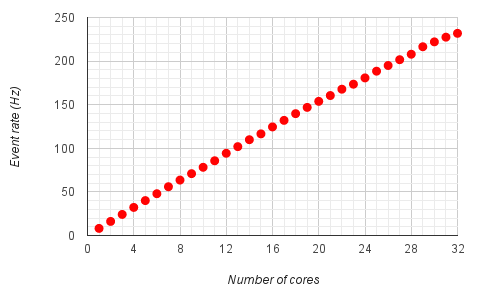
\includegraphics[width=\textwidth]{figures/coat-multicore}
    \end{minipage}%\hspace{2pc}%
    \begin{minipage}{0.48\textwidth}
      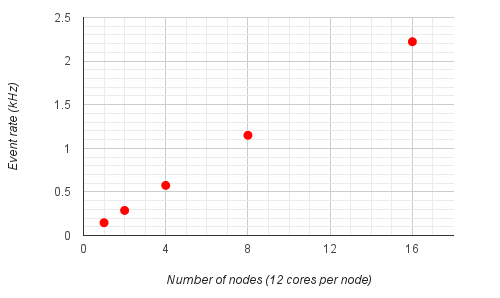
\includegraphics[width=\textwidth]{figures/coat-multinode}
    \end{minipage}
  \end{center}
  \caption{CLAS application scalability.}
  \label{fig:results}
\end{figure}

\section*{References}
\begin{thebibliography}{9}
  \bibitem{soa} Erl T 2007 \textit{SOA: Principles of Service Design} (Prentice Hall)
  \bibitem{xmsg} Gyurjyan V xMsg: General Purpose Publish-Subscribe Messaging System (unpublished)
  \bibitem{zmq} Hintjens P 2013 \textit{ZeroMQ: Messaging for Many Applications} (O'Reilly Media)
\end{thebibliography}

\end{document}
